\section{Auswertung}
\label{sec:Auswertung}

Die aufgenommenen Werte, sowie die um den Untergrund bereinigten Werte (siehe
Kapitel \ref{sec:untergrund}) sind in den Tabellen \ref{tab:messwerte1}
bis \ref{tab:messwerte3} dargestellt. Im Folgenden bezeichnet der Index 1 die
Messreihe mit der geringeren Heizrate und der Index 2 die Messreihe mit der
höheren Heizrate.

\begin{table}[htp]
	\begin{center}
    \caption{Messwerte mit und ohne Bereinigung um den Untergrund für beide Messreihen.}
    \label{tab:messwerte1}
		\begin{tabular}{cccccc}
		\toprule
			{$T_1$/°C} & {$I_1$/pA} & {$I_{1,bereinigt}$/pA} & {$T_2$/°C} & {$I_2$/pA} & {$I_{2,bereinigt}$/pA}\\
			\midrule
			-63,00 & 0,80 & 0,55 & -63,5 & 0,20 & -0,15\\
			-61,80 & 0,80 & 0,52 & -61,4 & 0,15 & -0,28\\
			-60,00 & 0,80 & 0,48 & -58,3 & 0,10 & -0,45\\
			-58,20 & 0,80 & 0,44 & -56,0 & 0,00 & -0,65\\
			-56,90 & 0,75 & 0,36 & -54,0 & 0,05 & -0,68\\
			-55,60 & 0,70 & 0,28 & -52,8 & 0,10 & -0,68\\
			-54,40 & 0,65 & 0,20 & -51,8 & 0,08 & -0,75\\
			-53,20 & 0,65 & 0,17 & -50,8 & 1,00 & 0,13\\
			-52,10 & 0,60 & 0,09 & -49,2 & 2,20 & 1,25\\
			-51,00 & 0,60 & 0,06 & -47,1 & 3,30 & 2,25\\
			-49,90 & 0,60 & 0,03 & -45,1 & 1,90 & 0,75\\
			-48,70 & 0,60 & -0,00 & -43,4 & 1,20 & -0,04\\
			-47,60 & 0,60 & -0,04 & -41,7 & 1,20 & -0,13\\
			-46,50 & 0,65 & -0,02 & -39,8 & 1,70 & 0,27\\
			-45,50 & 0,65 & -0,05 & -37,8 & 1,40 & -0,15\\
			-44,40 & 0,70 & -0,04 & -35,6 & 1,70 & 0,02\\
			-43,40 & 0,80 & 0,03 & -34,1 & 2,10 & 0,33\\
			-42,20 & 0,85 & 0,04 & -32,5 & 2,50 & 0,63\\
			-41,20 & 0,90 & 0,06 & -31,4 & 2,80 & 0,86\\
			-40,10 & 1,05 & 0,17 & -29,7 & 3,40 & 1,35\\
			-39,00 & 1,15 & 0,23 & -28,2 & 4,10 & 1,94\\
			-37,80 & 1,35 & 0,38 & -26,5 & 5,10 & 2,83\\
			-36,60 & 1,50 & 0,49 & -24,6 & 6,30 & 3,89\\
			-35,30 & 1,80 & 0,74 & -22,6 & 8,10 & 5,54\\
			-34,00 & 2,20 & 1,08 & -20,5 & 10,00 & 7,27\\
			-32,90 & 2,40 & 1,24 & -18,8 & 11,50 & 8,63\\
			-32,00 & 2,80 & 1,60 & -17,3 & 12,50 & 9,51\\
			-31,00 & 3,10 & 1,85 & -15,6 & 13,50 & 10,36\\
			-30,00 & 3,50 & 2,21 & -13,5 & 15,00 & 11,68\\
			-29,20 & 3,80 & 2,47 & -11,5 & 15,00 & 11,49\\
			-28,00 & 4,30 & 2,92 & -9,5 & 14,00 & 10,30\\
			-26,40 & 5,10 & 3,64 & -7,8 & 12,00 & 8,13\\
			-25,00 & 6,00 & 4,47 & -6,1 & 10,50 & 6,46\\
			-23,80 & 6,80 & 5,21 & -4,2 & 8,50 & 4,26\\
			-22,90 & 7,30 & 5,66 & -2,2 & 6,80 & 2,34\\
			-22,30 & 7,70 & 6,03 & -0,4 & 6,00 & 1,33\\
			-21,10 & 8,20 & 6,46 & 1,1 & 5,30 & 0,46\\
			-19,80 & 8,90 & 7,09 & 2,5 & 5,10 & 0,09\\
			-18,40 & 9,60 & 7,70 & 4,0 & 5,10 & -0,10\\
			-17,20 & 10,00 & 8,03 & 5,8 & 5,40 & -0,03\\
			-16,00 & 10,00 & 7,96 & 7,6 & 5,70 & 0,04\\
			-14,80 & 10,00 & 7,88 & 9,5 & 6,20 & 0,28\\
      \bottomrule
      \end{tabular}
    \end{center}
  \end{table}
  \begin{table}[htp]
  	\begin{center}
      \caption{Messwerte mit und ohne Bereinigung um den Untergrund für beide Messreihen (Fortsetzung).}
      \label{tab:messwerte2}
  		\begin{tabular}{cccccc}
  		\toprule
  			{$T_1$/°C} & {$I_1$/pA} & {$I_{1,bereinigt}$/pA} & {$T_2$/°C} & {$I_2$/pA} & {$I_{2,bereinigt}$/pA}\\
  			\midrule
			-13,50 & 9,30 & 7,10 & 11,3 & 6,60 & 0,43\\
			-12,50 & 8,60 & 6,33 & 13,2 & 7,10 & 0,65\\
			-11,40 & 7,70 & 5,35 & 15,1 & 7,50 & 0,76\\
			-10,10 & 7,10 & 4,66 & 16,8 & 7,90 & 0,90\\
			-8,30 & 6,50 & 3,92 & 18,5 & 8,20 & 0,93\\
			-6,80 & 5,70 & 3,01 & 20,2 & 8,60 & 1,04\\
			-5,60 & 5,00 & 2,21 & 21,8 & 9,00 & 1,17\\
			-5,00 & 4,30 & 1,46 & 23,3 & 9,00 & 0,91\\
			-4,20 & 3,80 & 0,90 & 24,7 & 9,50 & 1,15\\
			-2,90 & 3,70 & 0,69 & 26,3 & 9,60 & 0,96\\
			-1,80 & 3,60 & 0,49 & 27,9 & 9,60 & 0,65\\
			-0,80 & 3,60 & 0,40 & 29,6 & 9,90 & 0,62\\
			0,10 & 3,40 & 0,12 & 31,4 & 10,00 & 0,35\\
			0,70 & 3,30 & -0,03 & 33,3 & 10,30 & 0,25\\
			1,80 & 3,40 & -0,04 & 35,1 & 10,50 & 0,06\\
			3,80 & 3,70 & 0,06 & 36,9 & 10,50 & -0,35\\
			5,00 & 4,10 & 0,34 & 38,7 & 10,60 & -0,67\\
			5,80 & 4,20 & 0,36 & 40,3 & 10,70 & -0,95\\
			6,40 & 4,20 & 0,29 & 42,0 & 11,00 & -1,07\\
			7,10 & 4,20 & 0,22 & 43,7 & 11,10 & -1,40\\
			8,40 & 4,50 & 0,37 & 45,2 & 11,20 & -1,70\\
			9,70 & 4,80 & 0,53 & 46,7 & 11,20 & -2,10\\
			10,60 & 5,00 & 0,62 & 48.,0& 11,30 & -2,39\\
			11,40 & 5,00 & 0,52 & 49,7 & 11,00 & -3,15\\
			12,50 & 5,20 & 0,59 & 51,1 & 10,70 & -3,86\\
			13,80 & 5,50 & 0,73 & 52,7 & 10,30 & -4,74\\
			15,20 & 5,90 & 0,95 & 54,0 & 9,90 & -5,54\\
			16,20 & 6,10 & 1,01 & 55,4 & 9,20 & -6,68\\
			17,00 & 6,20 & 1,00 & 56,7 & 8,90 & -7,41\\
			17,90 & 6,20 & 0,88 & 57,9 & 7,60 & -9,10\\
			19,10 & 6,50 & 1,01 & - & - & -\\
			20,30 & 6,70 & 1,03 & - & - & -\\
			21,20 & 6,90 & 1,09 & - & - & -\\
			21,90 & 6,90 & 0,99 & - & - & -\\
			22,70 & 6,80 & 0,76 & - & - & -\\
			23,70 & 6,90 & 0,70 & - & - & -\\
			25,00 & 7,10 & 0,69 & - & - & -\\
			26,30 & 7,50 & 0,87 & - & - & -\\
			27,30 & 7,60 & 0,80 & - & - & -\\
			28,30 & 7,60 & 0,62 & - & - & -\\
			29,30 & 7,60 & 0,44 & - & - & -\\
			30,20 & 7,60 & 0,27 & - & - & -\\
      \bottomrule
      \end{tabular}
    \end{center}
  \end{table}

\begin{table}[htp]
	\begin{center}
    \caption{Messwerte mit und ohne Bereinigung um den Untergrund für beide Messreihen (Fortsetzung).}
    \label{tab:messwerte3}
		\begin{tabular}{cccccc}
		\toprule
			{$T_1$/°C} & {$I_1$/pA} & {$I_{1,bereinigt}$/pA} & {$T_2$/°C} & {$I_2$/pA} & {$I_{2,bereinigt}$/pA}\\
			\midrule
			31,30 & 7,60 & 0,06 & - & - & -\\
			32,30 & 7,70 & -0,03 & - & - & -\\
			33,40 & 7,90 & -0,05 & - & - & -\\
			34,60 & 8,10 & -0,10 & - & - & -\\
			35,70 & 8,20 & -0,23 & - & - & -\\
			36,70 & 8,30 & -0,35 & - & - & -\\
			37,80 & 8,50 & -0,39 & - & - & -\\
			38,80 & 8,60 & -0,52 & - & - & -\\
			39,70 & 8,70 & -0,63 & - & - & -\\
			40,80 & 8,90 & -0,69 & - & - & -\\
			41,80 & 9,00 & -0,84 & - & - & -\\
			42,90 & 9,10 & -1,01 & - & - & -\\
			44,20 & 9,30 & -1,15 & - & - & -\\
			45,40 & 9,50 & -1,27 & - & - & -\\
			46,50 & 9,50 & -1,57 & - & - & -\\
			47,40 & 9,40 & -1,92 & - & - & -\\
			48,30 & 9,10 & -2,48 & - & - & -\\
			49,70 & 9,00 & -2,99 & - & - & -\\
			51,00 & 9,00 & -3,38 & - & - & -\\
			52,20 & 8,60 & -4,15 & - & - & -\\
			53,20 & 8,30 & -4,77 & - & - & -\\
			54,20 & 7,90 & -5,50 & - & - & -\\
			55,30 & 7,50 & -6,27 & - & - & -\\
			56,50 & 7,00 & -7,19 & - & - & -\\
		\bottomrule
		\end{tabular}
	\end{center}
\end{table}

\subsection{Bestimmung der tatsächlichen Heizraten}
Zunächst sollen die tatsächlichen Heizraten bestimmt werden. Die angestrebten
Heizraten waren $1{,}2\,$K/min und 2\,K/min. Die tatsächlichen Heizraten lassen
sich mithilfe einer Ausgleichsrechnung der Form
\begin{equation*}
  f(T)=aT+n
\end{equation*}
berechnen. Dabei wird der bei der niedrigsten Temperatur gemessene Wert als bekannter
Punkt festgelegt. Die Heizrate ergibt sich aus der Steigung der Geraden. Sie beträgt
\begin{align*}
  b_1&=\SI{1.1339(0024)}{\kelvin\per\minute}= \SI{0.01890(00004)}{\kelvin\per\second}\,, \\
  b_2&=\SI{1.7587(0033)}{\kelvin\per\minute}= \SI{0.02931(00005)}{\kelvin\per\second}\,.
\end{align*}
Die Messwerte und die Ausgleichsfunktionen sind in den Abbildungen \ref{fig:heiz1}
und \ref{fig:heiz2} zu sehen.

\begin{figure}
  \centering
  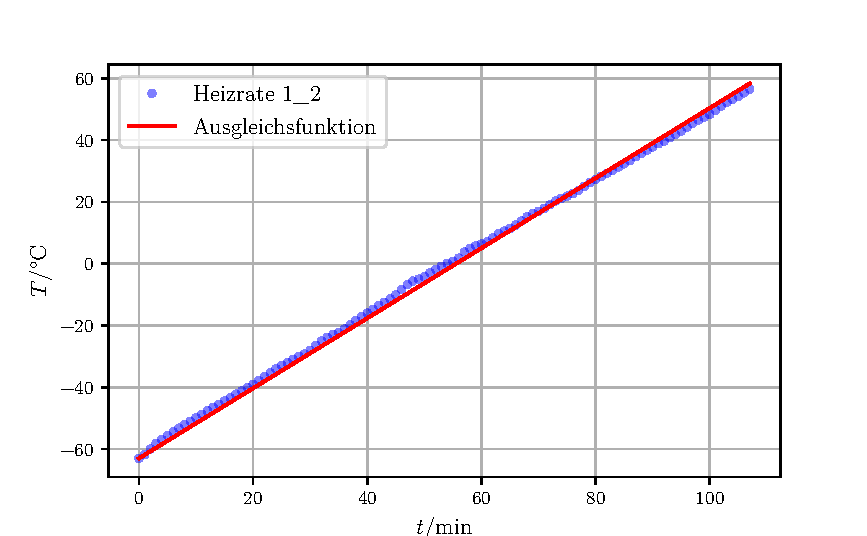
\includegraphics[width=\textwidth]{build/interpol_1_2.pdf}
  \caption{Messwerte und lineare Ausgleichsrechnung zur Bestimmung der tatsächlichen
  Heizrate für die Messreihe mit niedrigerer Heizrate.}
  \label{fig:heiz1}
\end{figure}
\begin{figure}
  \centering
  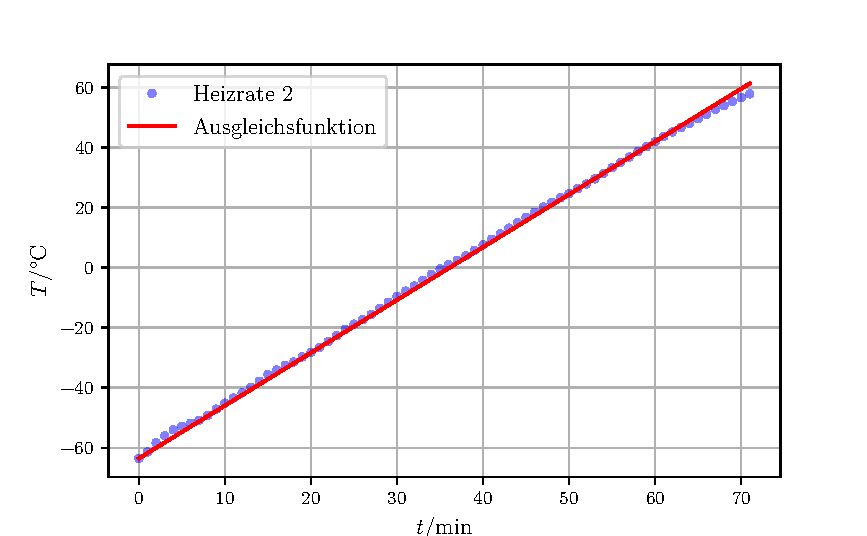
\includegraphics[width=\textwidth]{build/interpol_2.pdf}
  \caption{Messwerte und lineare Ausgleichsrechnung zur Bestimmung der tatsächlichen
  Heizrate für die Messreihe mit höherer Heizrate.}
  \label{fig:heiz2}
\end{figure}


\subsection{Bestimmung und Abzug des Untergrundes}
\label{sec:untergrund}

Zur Bestimmung des Untergrundes müssen zunächst Werte für die Minima des Stroms per Hand gefunden
werden. Für die gefundenen Werte wird anschließend eine Ausgleichsrechnung der
Form
\begin{equation*}
  f(T)=a e^{bT} +c
\end{equation*}
durchgeführt. Dabei sind alle Werte, die in der Ausgleichsrechnung verwendet werden,
per Hand gefundene Werte, die annähernd den Verlauf einer Exponentialfunktion
widerspiegeln. Es ergeben sich die Parameter
\begin{align*}
  a_1&=\SI{3.9(05)}{\pico\ampere}  \,,\\
  b_1&=\SI{0.024(0005)}{\per\kelvin}  \,,\\
  c_1&=\SI{-0.6(05)}{\pico\ampere}  \,,\\
  a_2&=\SI{6(4)}{\pico\ampere}  \,,\\
  b_2&=\SI{0.018(018)}{\per\kelvin}  \,,\\
  c_2&=\SI{-2(4)}{\pico\ampere}  \,.
\end{align*}
Es ist erkennbar, dass die Unsicherheiten dieser Parameter sehr groß sind.
Die Ausgleichsfunktionen für den Untergrund, sowie die für die Ausgleichsrechnungen
verwendeten Werte sind in den Abbildungen \ref{fig:depol1} und \ref{fig:depol2} zu sehen.
Außerdem sind dort die um den Untergrund bereinigten Daten dargestellt, mit denen auch
im Folgenden weitergerechnet wird.

\begin{figure}
  \centering
  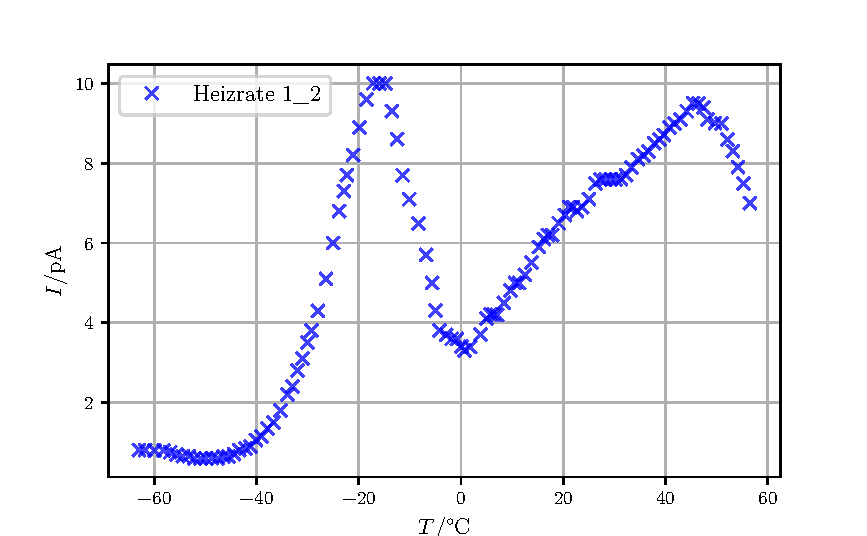
\includegraphics[width=\textwidth]{build/depolarisationskurve_1_2.pdf}
  \caption{Messwerte, sowie Ausgleichsrechnung für den Untergrund aus den markierten Werten
  und um den Untergrund bereinigte Daten für die Messreihe mit der niedrigeren Heizrate.}
  \label{fig:depol1}
\end{figure}
\begin{figure}
  \centering
  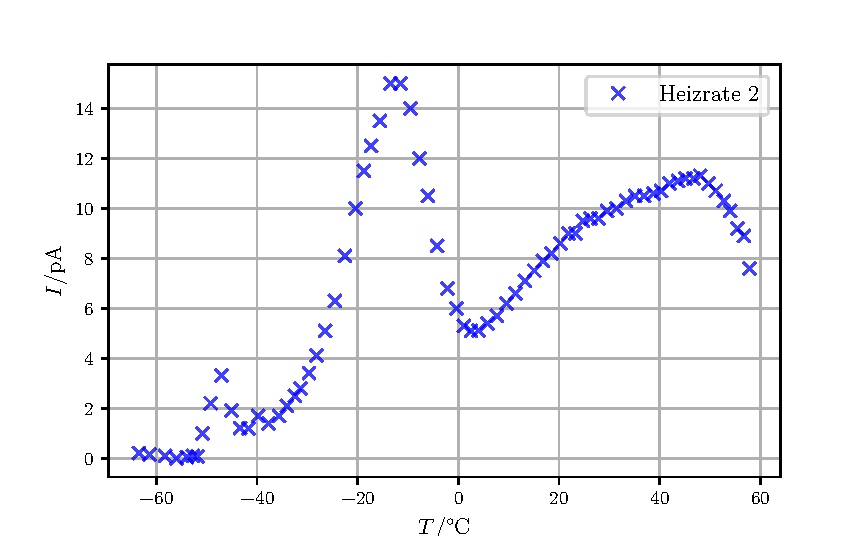
\includegraphics[width=\textwidth]{build/depolarisationskurve_2.pdf}
  \caption{Messwerte, sowie Ausgleichsrechnung für den Untergrund aus den markierten Werten
  und um den Untergrund bereinigte Daten für die Messreihe mit der höheren Heizrate.}
  \label{fig:depol2}
\end{figure}

\subsection{Bestimmung der Aktivierungsenergie über die Stromdichte}

Es wird die Näherung aus Gleichung \eqref{eqn:naeherung} verwendet. Wenn nun $i(T)$
logarithmiert wird, erhält man
\begin{equation*}
  \ln(i(T))=-\frac{W}{k_B T} + const =a\cdot \frac{1}{T} +b  \,.
\end{equation*}
Es wird nun $\ln(i(T))$ gegen $1/T$ aufgetragen und es wird eine lineare Ausgleichsrechnung
durchgeführt. Dabei werden zunächst die Werte vom ersten Minimum bis zum erstem Maximum
des Depolarisationsstroms verwendet. Anschließend werden davon die Werte ausgewählt, die
noch einen annähernd linearen Verlauf zeigen. Die Werte für höhere Temperaturen werden
nicht berücksichtigt, da die oben genannte Näherung nur bei geringen
Temperaturen gültig ist.

Die Parameter
der Ausgleichsrechnungen ergeben sich zu
\begin{align*}
  a_1&=\SI{-7.6(4)e+3}{\per\kelvin} \,, \\
  b_1&=\SI{31.8(16)}{}  \,, \\
  a_2&=\SI{-9.0(7)e+3}{\per\kelvin} \,, \\
  b_2&=\SI{37.1(29)}{}  \,.
\end{align*}
Die Aktivierungsenergien können damit über $W=-ak_B$ zu
\begin{align*}
 W_1&=\SI{1.04(06)e-19}{\joule}= \SI{0.652(034)}{\eV}  \,, \\
 W_2&=\SI{1.24(10)e-19}{\joule}=\SI{0.77(06)}{\eV} \,.
\end{align*}
bestimmt werden.

Die Werte und die Ausgleichsrechnung sind in den Abbildungen \ref{fig:fit1} und
\ref{fig:fit2} dargestellt.

\begin{figure}
  \centering
  \includegraphics[width=\textwidth]{build/fit1.pdf}
  \caption{Messwerte und lineare Ausgleichsrechnung zur Bestimmung der Aktivierungsenergie für
  die Messreihe mit der niedrigeren Heizrate.}
  \label{fig:fit1}
\end{figure}
\begin{figure}
  \centering
  \includegraphics[width=\textwidth]{build/fit2.pdf}
  \caption{Messwerte und lineare Ausgleichsrechnung zur Bestimmung der Aktivierungsenergie für
  die Messreihe mit der höheren Heizrate.}
  \label{fig:fit2}
\end{figure}

\subsection{Bestimmung der Aktivierungsenergie aus dem Polarisationsansatz}
